\chapter{Basic Procedure and System Characteristics}
\label{ch:basicprocedure}
% ##################################################################################################################
\hfill \textbf{Author:} Andreas Horni 

\begin{center} 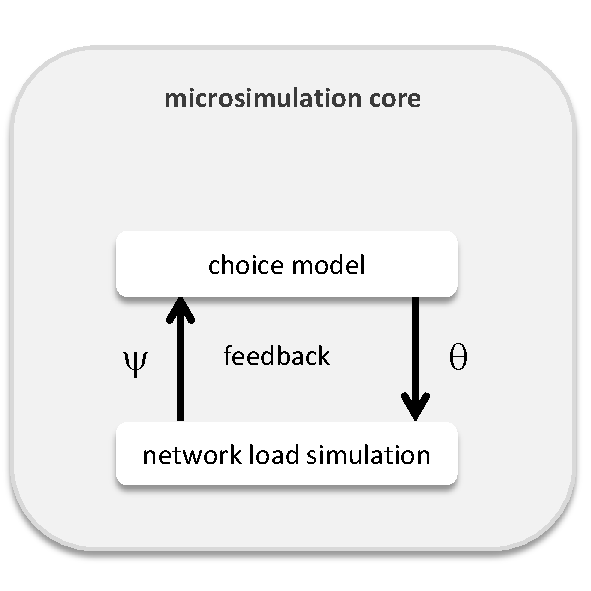
\includegraphics[width=0.3\textwidth, angle=0]{understanding/figures/fixedpoint.pdf} \end{center}

% ##################################################################################################################
\section{Basic Procedure}
The basic procedure of equilibrium-based microsimulations, such as MATSim or TRANSIMS is depicted in Figure \ref{fig:maxUtf}. A comprehensive (discrete) choice model is applied to a population for a specific choice situation. The choices are forwarded to a network load simulation (sometimes also called the physical simulation or mobility simulation). This network simulation can also contain other infrastructure elements than the road infrastructure, for example the facilities. It takes into account constraints, such as network capacities. Generalized travel costs, calculated based on the simulation, are fed back to the choice model. The choice model is also subject to constraints such as opening hours. The microsimulation is instantiated by census data for the population, travel surveys to estimate the models and infrastructure information to define the constraints. This instantiation or application is described for the MATSim Zürich scenario by  \citet[][]{HorniEtAl_TechRep_IVT_2011_a}. %In a very general sense, utility-based transport microsimulations do utility-maximization subject to constraints following the discrete choice methodology.

% ----------
\createfigure%
{Basic procedure of transport microsimulations}%
{Basic procedure of transport microsimulations}%
{\label{fig:maxUtf}}%
{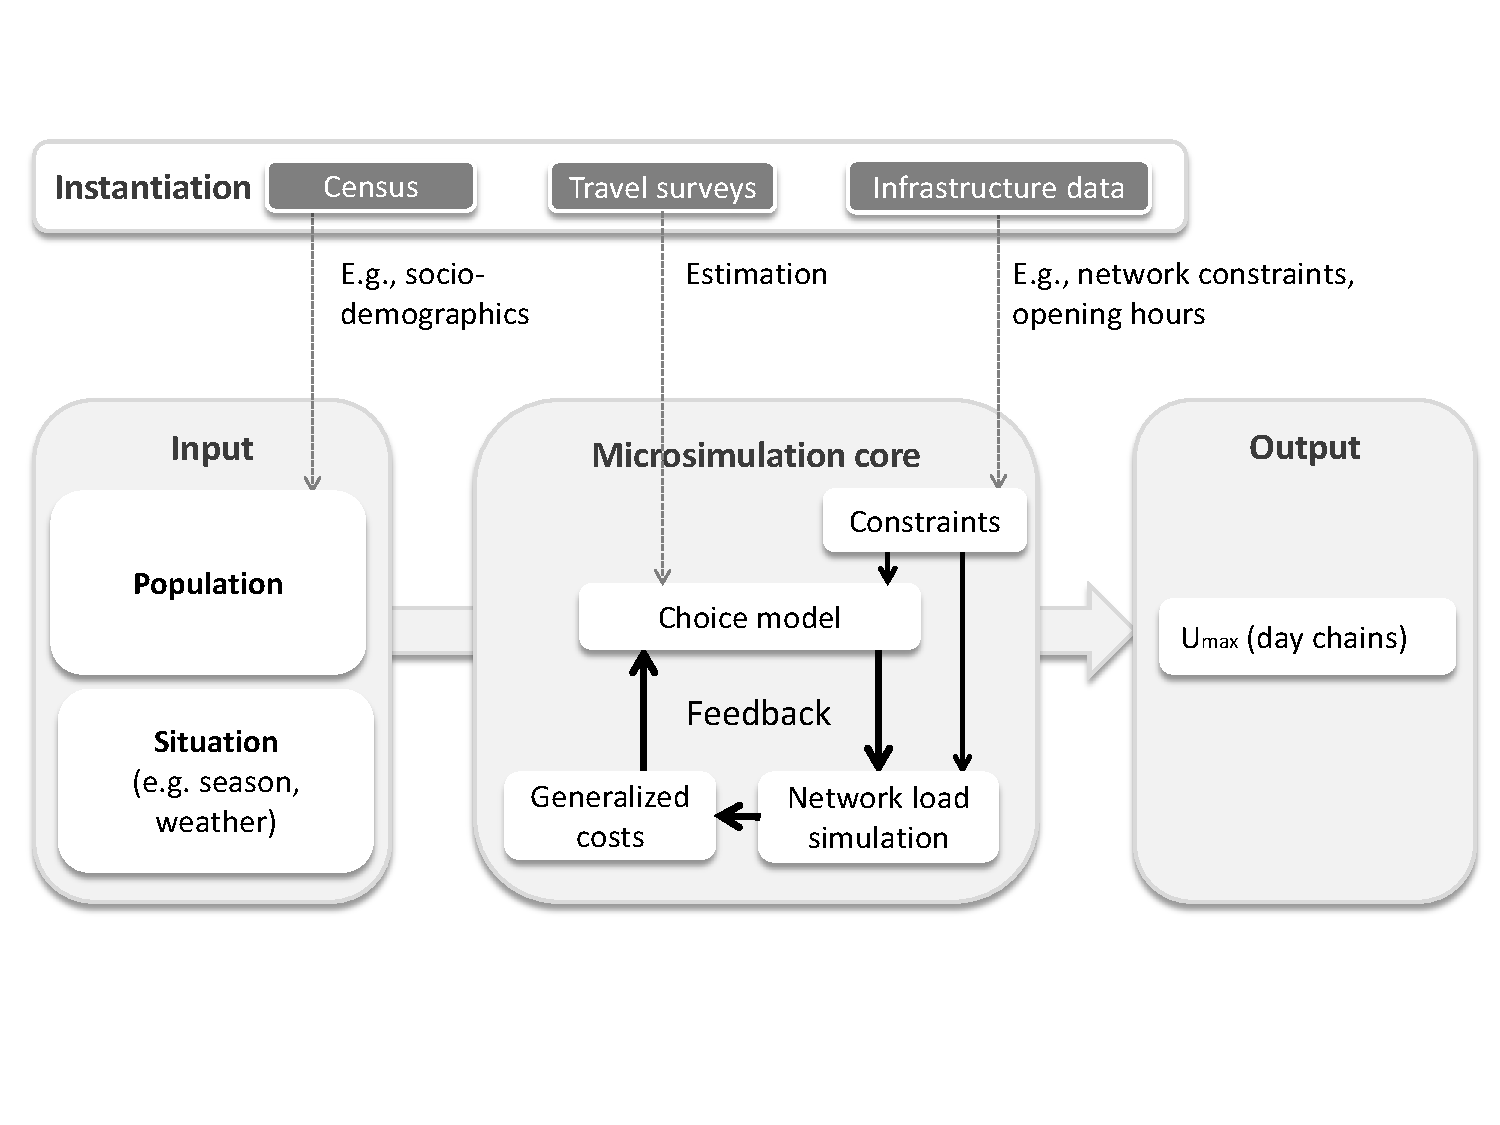
\includegraphics[width=0.99\textwidth, angle=0]{understanding/figures/maxUtf.pdf}}%
{}

% ----------

The cycle in the middle of Figure \ref{fig:maxUtf} represents a systematic relaxation process \citep[e.g.,][Figure 1.3]{Balmer_PhDThesis_2007}. In MATSim, the interpretation of the relaxation procedure is unclear. Sometimes the relaxation process is ascribed a behavioral interpretation, for example, day-to-day learning, where also the transition process and not only the final equilibrium has a meaning \citep[][p.128]{LiuEtAl_TransResA_2006}, \citep[][p.523]{NagelBarrett_IJMPC_1997}. An opposite perspective exists, where the relaxation procedure is just a numerical method to compute the Nash equilibrium without behavioral basis of the transitions.

To reveal similarities with known mathematical problems and their solution approaches a more abstract formulation can be established. 

The choice model draw is given as follows.
\begin{equation}
\label{eq:choiceModel}
\theta = h_0(\beta, y, \epsilon, \psi),
\end{equation}
where $\theta$ are the choices, $h_0$ is the choice model function, $\beta$ are the choice model coefficients, $\psi$ are the generalized costs given by the infrastructure conditions (e.g., network conditions), $y$ are further parameters such as the age of the decision maker and $\epsilon$ denotes the random error terms. 

Equilibrium-based transport microsimulations go beyond a single draw from a choice model. The parameters, such as the travel times, are an \emph{endogenous} component of these microsimulations. The circular relation between choices and the generalized costs can be written as a (usually non-linear) system of equations (see also Figure \ref{fig:fixedpoint}): 
\begin{equation}
\label{eq:initialSystem}
\begin{cases}
\theta = h_0(\beta, y, \epsilon, \psi) \\
\psi = h_1(\theta) 
\end{cases}
\end{equation}
where $\theta$ are the choices, $\psi$ are the generalized costs and $h_0$ and $h_1$ are mathematical maps. In microsimulations $h_0$ is implemented by the choice models and $h_1$ is the network loading simulation plus the succeeding conversion of infrastructure conditions into generalized costs. 

This can be rewritten as
\begin{equation}
\theta = h_0(\beta, y, \epsilon, h_1(\theta))
\end{equation}
%
or in a more general form:
%
\begin{equation}
\label{eq:phi}
\theta = \varphi(\theta, \beta, y, \epsilon) %f(\theta) = \varphi(\theta, \beta, y, \epsilon)
\end{equation}
%
%
% ----------
\createfigure%
{Fixed point problem}%
{Fixed point problem}%
{\label{fig:fixedpoint}}%
{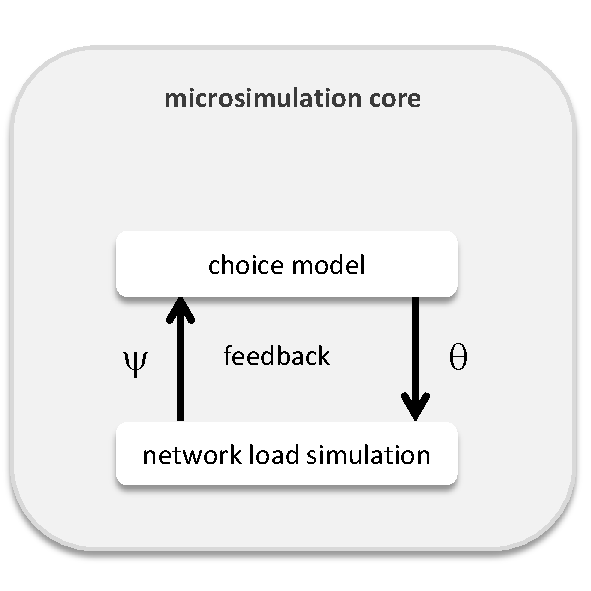
\includegraphics[width=0.4\textwidth, angle=0]{understanding/figures/fixedpoint.pdf}}%
{}
%
% ----------
%
This is a fixed point problem (see e.g., \citet[][p.6]{RamaduraiUkkusuri_TechRep_RPI_2008}, \citet[][]{BierlaireCrittin_TransScience_2006, KaufmanEtAl_TransResC_1998, RamaduraiUkkusuri_NSE_2010}). The fixed points are found by iteratively applying Equation \ref{eq:phi}. In the microsimulation context, \emph{iteratively}, the outcomes of the comprehensive choice model are directed to a network load simulation, whose outcomes (the infrastructure conditions) are in turn fed back to the choice model. But naively doing this most probably leads to very bad convergence behavior.

From numerics it is known that fixed point problems can be transformed such that convergence behavior is improved. This is explained with an example. In numerics root finding problems given as $f(x)=0$ are often transformed into fixed point problems as
\begin{equation}
\label{eq:fpf}
x=g(x)
\end{equation}
where the fixed points are the solutions of the root finding problem. As fixed point problems can be transformed, infinitely many possibilities exist for the choice of $g(.)$. For example the root finding problem $f(x)=x^2-2x-3=0$ can be transformed by using $g_0(x)=\sqrt{2x+3}$ or $g_1(x)=\frac{3}{x-2}$ or $g_2(x)=\frac{x^2-3}{2}$ to name a few. The choice of $g(.)$ thereby has a crucial impact on the convergence behavior, i.e., dependent on the form of $g(.)$ and the initial point $\theta_0$ the iterations may converge to a fixed point with different speed, are attracted by an orbit or may also move through the state space in a completely chaotic manner. In the example above, starting from $x_0=4$, $g_0(x)$ converges, $g_1(x)$ also converges but slower and $g_2(x)$ diverges. In numerics, the Picard method \citep[][p.2ff]{Vogt_TechRep_IfMath_2001} is improved by e.g., the Newton-Raphson method \citep[][p.28ff]{Vogt_TechRep_IfMath_2001}, which employs an efficient mapping for $g(.)$. 

A very similar approach is maybe productive for transport modeling; $\varphi(.)$ (which corresponds to $g(.)$) should be chosen reasonable, such that fixed points are found efficiently.

In first generation models, the fixed points are searched by implementing $\varphi(.)$ with iterative numerical algorithms such as the \emph{method of successive averages} (MSA) \citep[][p.342f]{OrtuzarWillumsen_2001} or the Frank-Wolfe algorithm \citep[][]{FrankWolfe_NRLQ_1956}, \citep[see also][p.4]{CorreaStier_Cochran_2010}. Every person searches its optimum subject to competition leading to an equilibrium state. This is achieved in the MSA by moving a certain share of the flow to the cheapest route, while taking it away from the remaining routes per OD-relation. For first generation models, much is known about existence, stability, uniqueness and computation of fixed points. Thus, by continuing the lines of the first generation models, one can hope to produce something reasonable also for second generation models, but this has to be investigated further. As shown in Section \ref{sec:co-ev}, a possible implementation of $\varphi(.)$ for MATSim is a co-evolutionary algorithm, which, in practice, has shown to efficiently lead to behaviorally sound fixed points.

% ##################################################################################################################
\section{System Characteristics}
% ##################################################################################################################
\subsection{Aggregate Traffic Flow Characteristics}
MATSim's aggregate traffic flow characteristics were analyzed in the common form of the macroscopic fundamental diagram. Some investigations additionally derived MATSim's (implicit) the volume-delay function \citep[][]{HorniMontini_STRC_2013}.

Some simulation investigations had problems to reproduce the complete MFD (project NetCap, personal communication, 2014), in particular, the high density region. They used mobism versions without the backward moving gaps feature. Other studies, based on DEQSim and JDEQSim respectively, which both \emph{do} include \emph{back moving gaps}, were able to generate realistic MFDs. 

\citet[p.81ff][]{Simoni_MastersThesis_2013} investigate MATSim's ability to model macroscopic characteristics with a four link ring scenario. He found considerable influence of the backward moving gaps speed on the form of the MFD. \citet[][]{CharyparEtAl_TRB_2009} also use a circular toy scenario. They also found the typical trapezoidal form for a broad range of network resolutions.

Natural conclusion here is, that back moving gaps are essential for generating a realistic MFD, in other words to realistically model to complete range of traffic conditions. Backward moving gaps are re-included in the default MATSim mobsim (qsim). 

% ##################################################################################################################
\subsection{Results Variability}
\label{sec:variability}
Microsimulation system design as well as concrete microsimulation studies require specification of the measures of interest \footnote{
Formal system specification (and verification) is discussed e.g., in \citet[][]{FisherWooldridge_IJCIS_1997, BourahlaBenmohamed_ENTCS_2005}. 
}. For microsimulation design, they need to be general and broadly available, count data are an example. For specific experiments and purposes other measures might be added; \citet[][]{Kitamura_TMIP_1996}, for example, lists measures relevant for emissions modeling. Considering their scale is important for model development, but a certain lack of research exists in this regard. \citet[][Section 2.2]{NagelAxhausen_TechRep_IVT_2001}, for example, say: ``Another question regarding scales is which scale is necessary to answer which question. There is wide-spread intuition but currently little hard knowledge. Rules-of-thumb, such as to include one level of resolution below the level of interest, are just rule-of-thumb.'' 

Scale of the measures of interest is also relevant for results production, as different scales or resolution levels usually lead to different levels of \emph{variability} and, thus, to different study costs in terms of required computation effort. Transport microsimulations are usually stochastic. Randomness is, for example, introduced by the error terms of discrete choice models, a common component in utility-based microsimulations. This leads to random variability in results. Parameters or population statistics, such as averages, thus, need to be estimated by random sampling. Microsimulations are thus essentially a sampling tool \citep[][]{WolfDA_CSP_2001}, where one run represents one sample unit (in statistical terms one \emph{realization of a random variable}). This makes clear, that the whole toolbox used for other statistical methods, must be applied also here. As a first step, required sample size---here, the number of runs---to ensure a given confidence in the calculated averages needs to be calculated. In this context, variability is often seen as something tedious, because higher variability leads to larger minimal sample sizes, with usually relatively high costs per sample point. But, this view falls short. Clearly, unobserved variability---modeled as random variability---should be replaced to the extent possible (by explaining it). However, when looking at the very large proportion of temporal variability actually present in reality (Figure \ref{fig:counts}), a substantial part of this variability is---even if it was actually explicable---much more efficiently handled by including randomness, as model complexity would be prohibitively large otherwise. In this sense, microsimulations are a tool to capture these real-world fluctuations \citep[][p.11]{NewmanMEJBarkema_1999}, \citep[][p.704]{EsserNagel_Hensher_2001}. This means also that the focus should not only be on averages, but also on variance incorporated in the calculations of statistical confidence. The following sections broaden the microsimulation variability analysis.

Multiple possibilities to categorize microsimulations variability exist; some categories are described by \citet[][]{HorniEtAl_TechRep_IVT_2011_b}. Often a distinction between endogenous (model) variability and exogenous (input) variability is made. Equally suitable one can distinguish systematic and random variability. The experiments reported below mainly focus on \emph{random, endogenous} model variability. Random variability stems from inherently random choices and from actually systematic choices not recognized as systematic by the modeler.

MATSim variability was investigated by \citet[][]{HorniEtAl_TechRep_IVT_2011_b, HorniEtAl_STRC_2011, Dayte_TechRep_IVT_2012} coming to the conclusion that at the population level, as expected, there is little variability between simulation results. Little variability exists likewise for \emph{daily} volumes as shown in Figures \ref{fig:linkVolumesAWTVInterScatter} and \ref{fig:linkVolumesInterAWTV200} (with a different visualization), which is consistent with previous work. However, the variability for \emph{hourly} volumes is an issue as shown in Figures~\ref{fig:linkVolumesHour17-18InterScatter} and Figure~\ref{fig:linkVolumesInter200} (with a different visualization).

To interact these substantial simualtion variability with variability observed in reality, \citet[][]{HorniEtAl_STRC_2011} looked at real-world link volumes given for both, the complete year and single months, meaning that a single point in the box plot represents temporal variability of a single network link, either for the whole year, or for a specific month. The hours 11-12 and 17-18 are shown as examples in Figure~\ref{fig:counts}, where similar patterns could be observed for all hours. The plots allow the conclusion that also in reality variability is also substantial.

Further MATSim investigations are reported by \citet[][]{Hackney_PhDThesis_2009, Neumann_PhDThesis_2014}.

\createfigure%
{Simulated link volumes}%
{Simulated link volumes}%
{\label{fig:linkVolumes}}%
{%
  \createsubfigure%
  {Daily Volumes: : Inter-run Variability}%
	{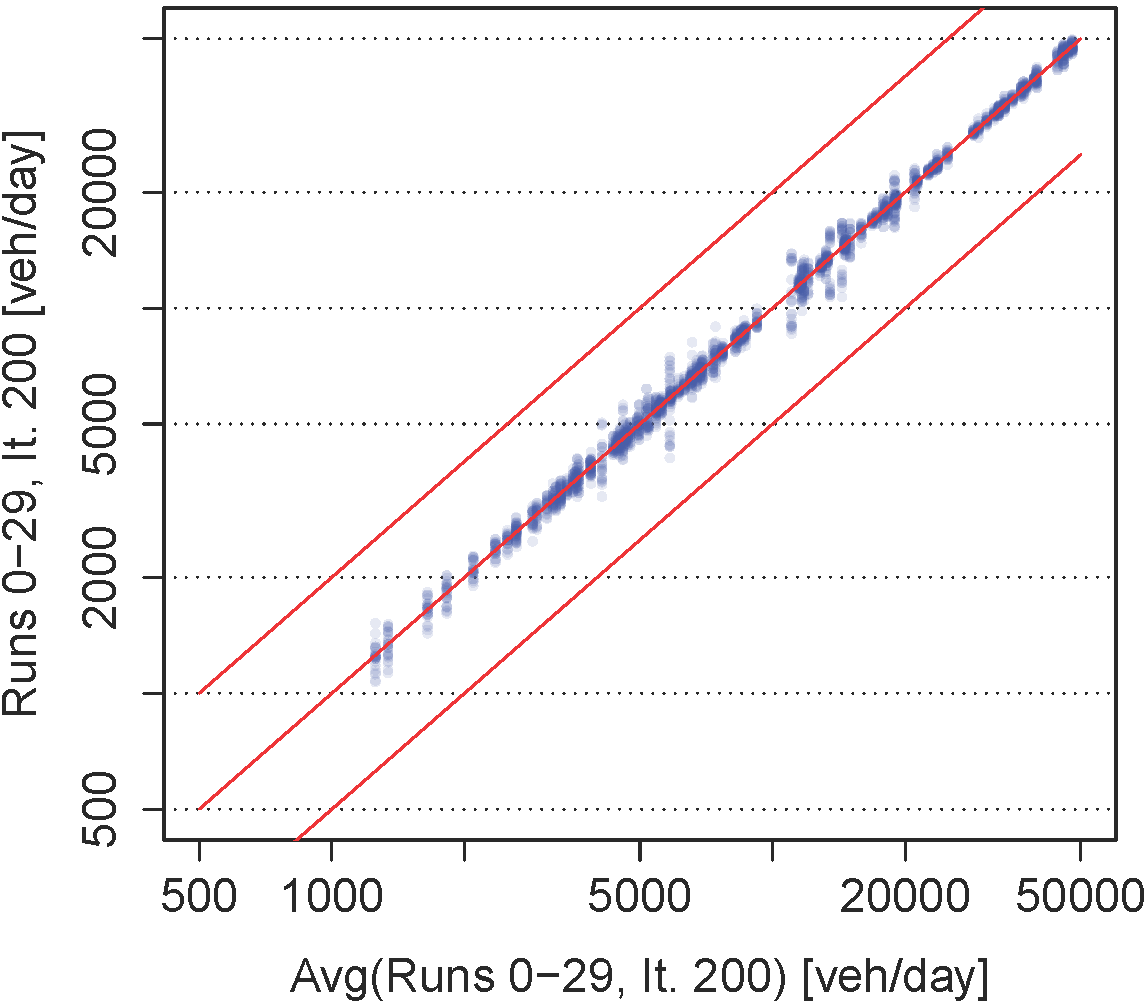
\includegraphics[width=0.49\textwidth]{understanding/figures/var/linkVolumesAWTVInterScatter.png}}%
	{\label{fig:linkVolumesAWTVInterScatter}}%
  {}%
	\createsubfigure%
  {Simulated Daily Volumes: Inter-run Variability, Runs 0-29, Iteration 200}%
	{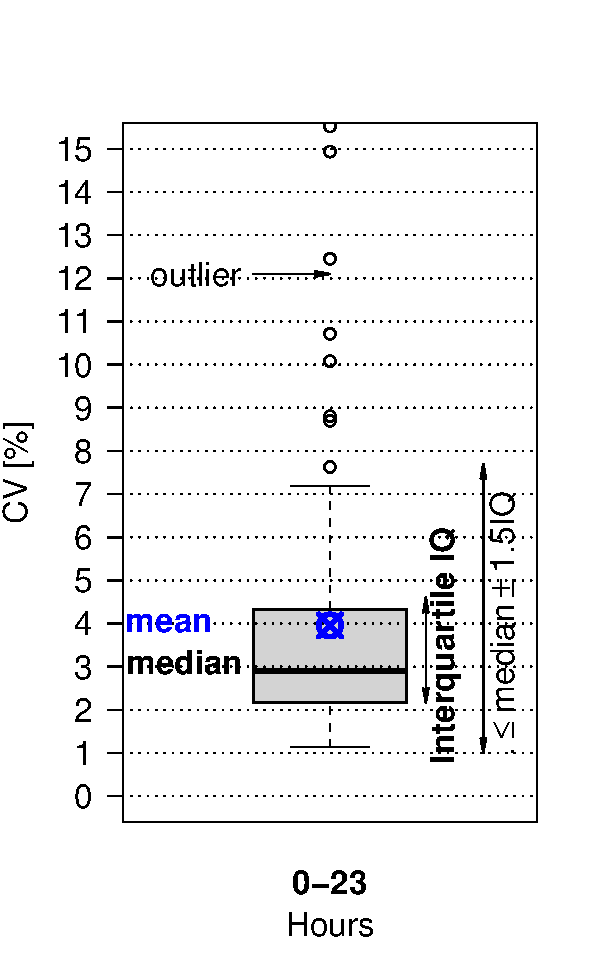
\includegraphics[width=0.4\textwidth]{understanding/figures/var/linkVolumesInterAWTV200.pdf}}%
	{\label{fig:linkVolumesInterAWTV200}}%
  {}%
  \createsubfigure%
  {Hourly Volumes (Hour 17-18), Inter-run Variability}%
	{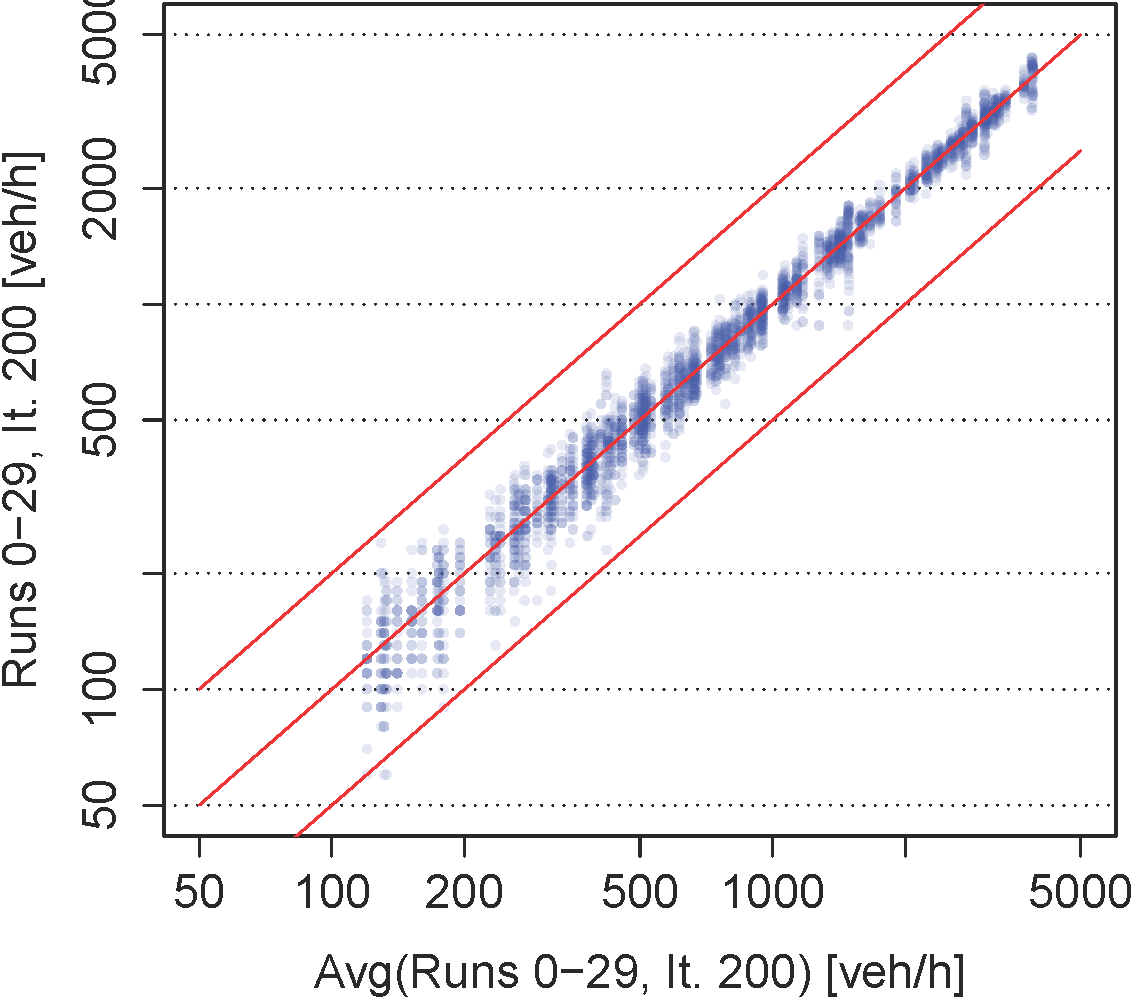
\includegraphics[width=0.49\textwidth]{understanding/figures/var/linkVolumesHour17-18InterScatter.png}}%
	{\label{fig:linkVolumesHour17-18InterScatter}}%
  {}%
	\createsubfigure%
  {Simulated Hourly Volumes: Inter-run Variability, Runs 0-29, Iteration 200}%
	{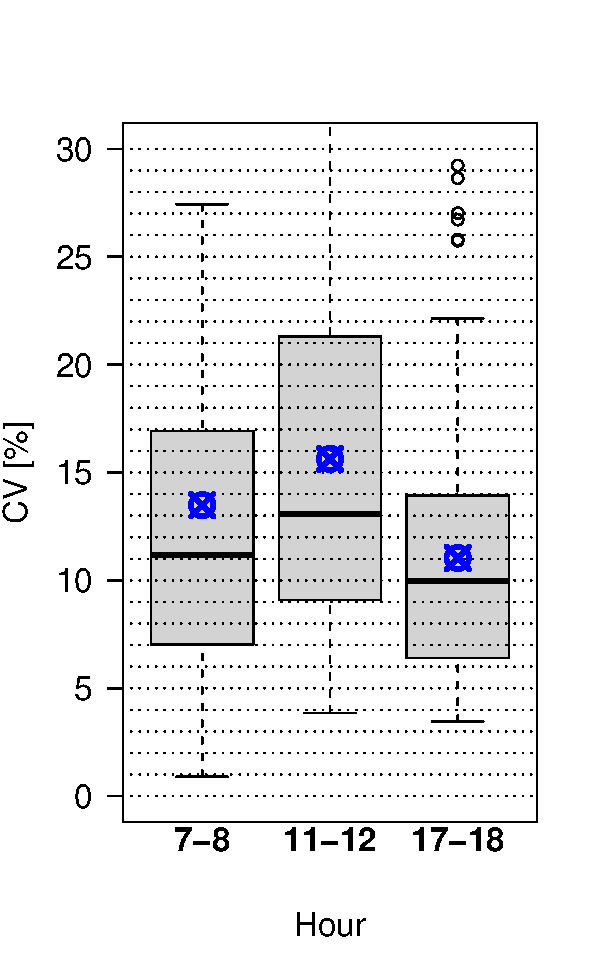
\includegraphics[width=0.4\textwidth]{understanding/figures/var/linkVolumesInter200.pdf}}%
	{\label{fig:linkVolumesInter200}}%
  {}%
}%
{} 

\createfigure%
{Measured volumes}%
{Measured volumes}%
{\label{fig:counts}}%
{%
	\createsubfigure%
  {Daily Volumes}%
	{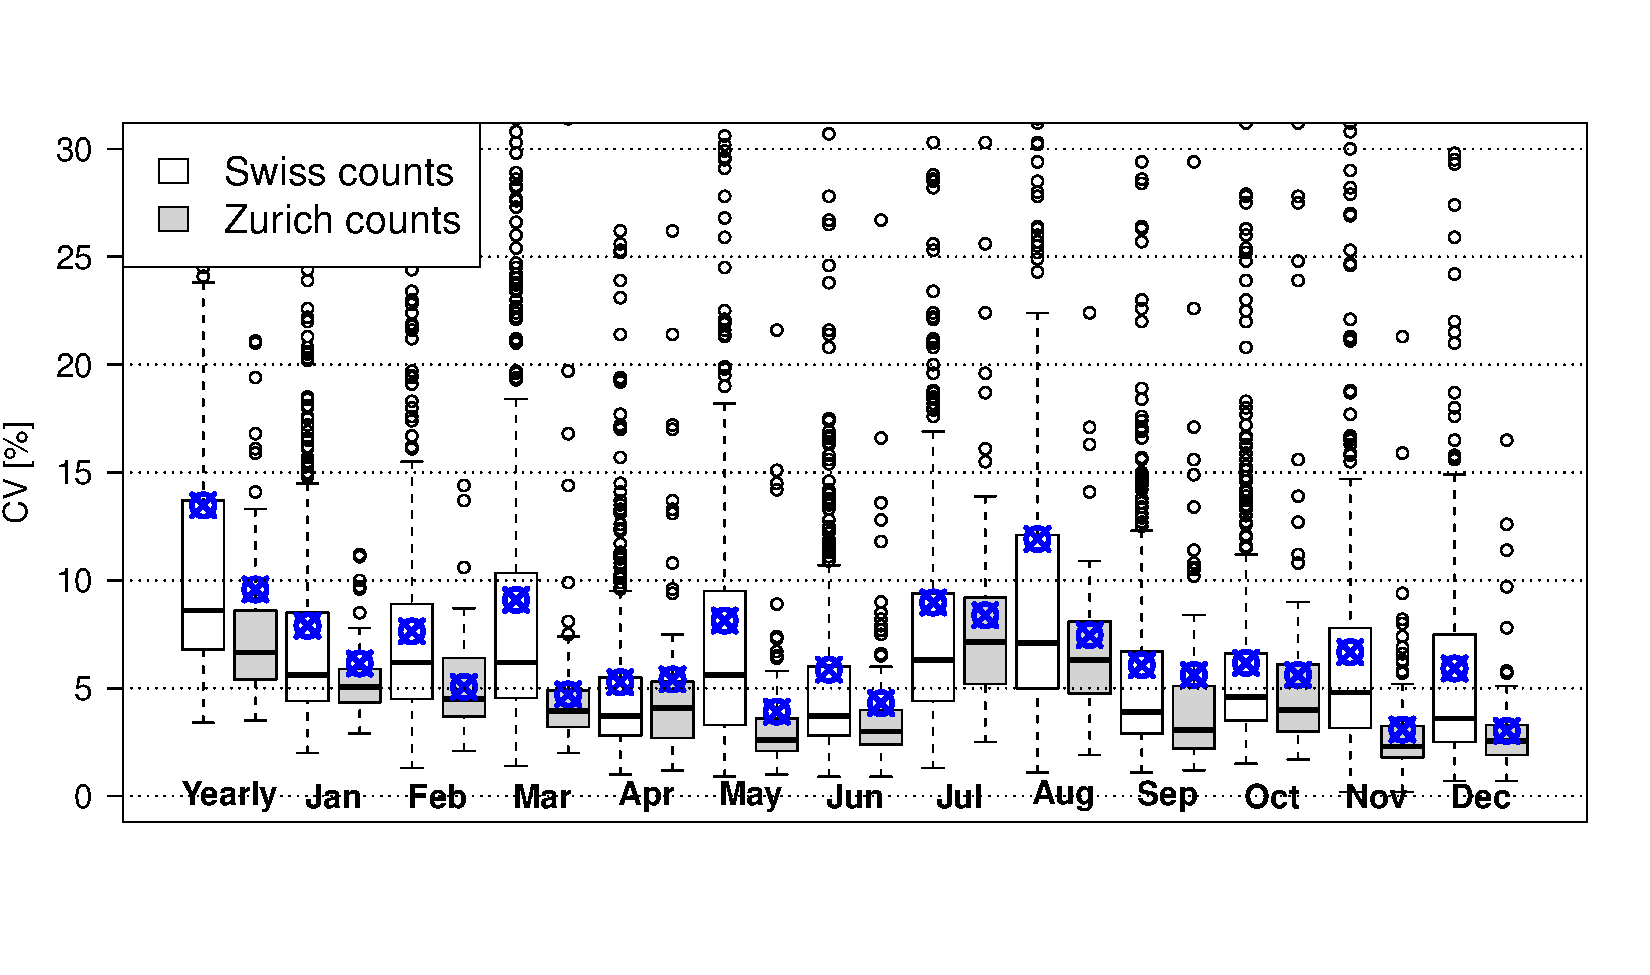
\includegraphics[width=0.8\textwidth]{understanding/figures/var/countsDaily.pdf}}%
	{\label{fig:countsDaily}}%
  {}%
  \createsubfigure%
  {11:00-12:00}%
	{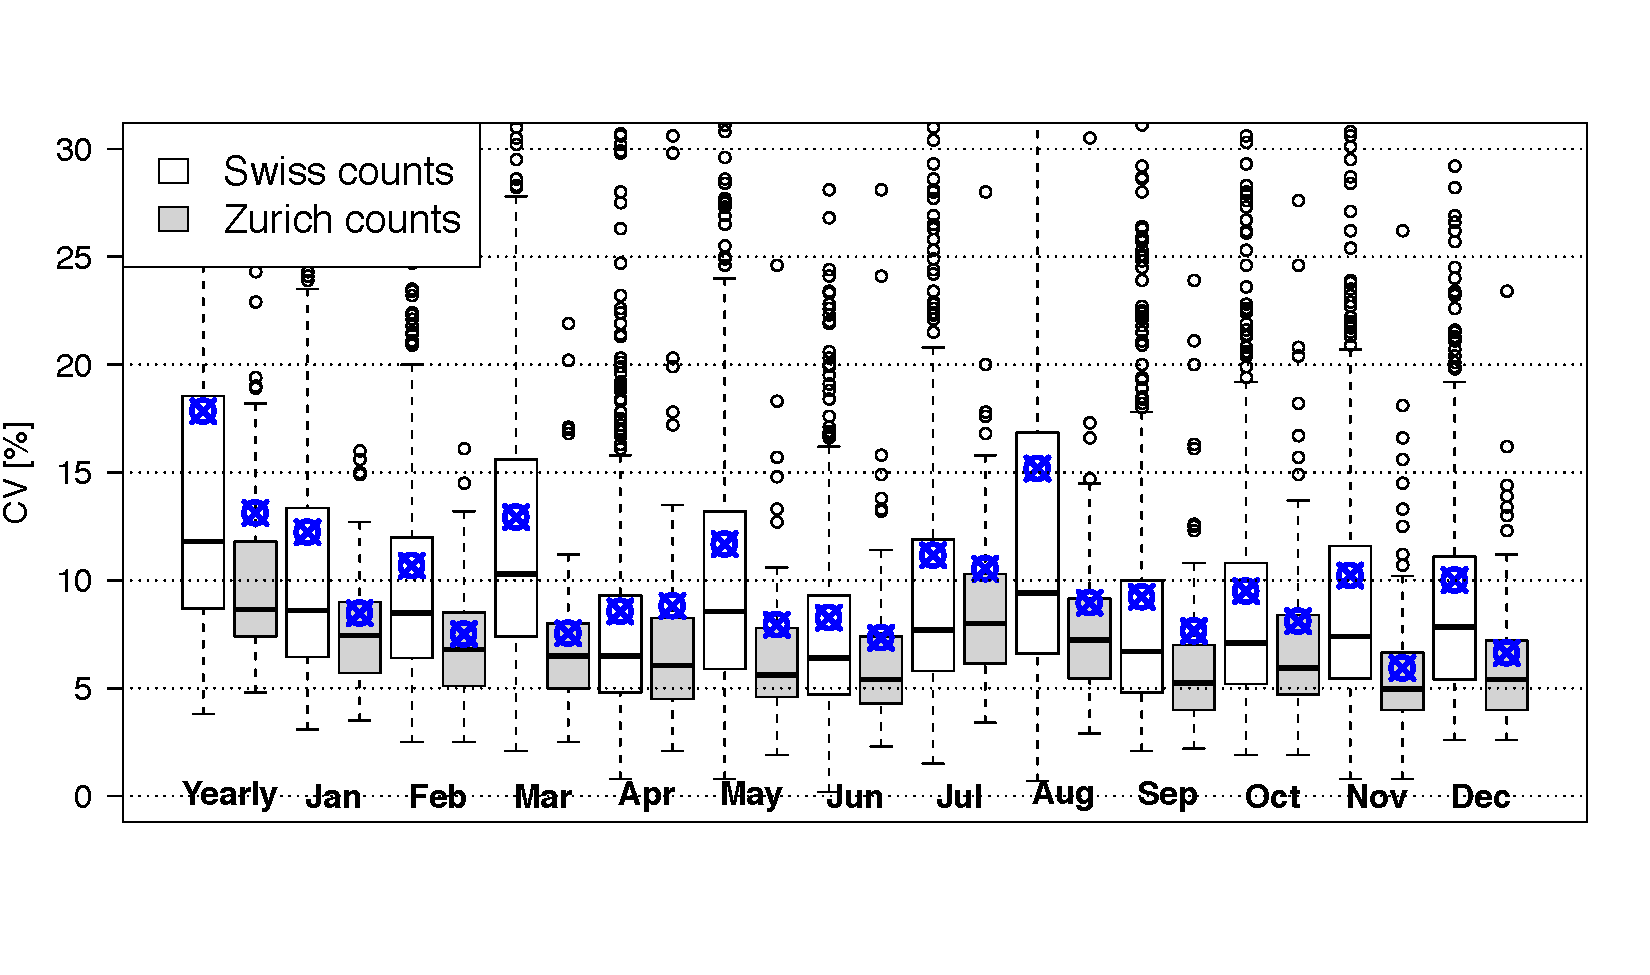
\includegraphics[width=0.8\textwidth]{understanding/figures/var/counts11-12.pdf}}%
	{\label{fig:H1112}}%
  {}%
 	\createsubfigure%
  {17:00-18:00}%
	{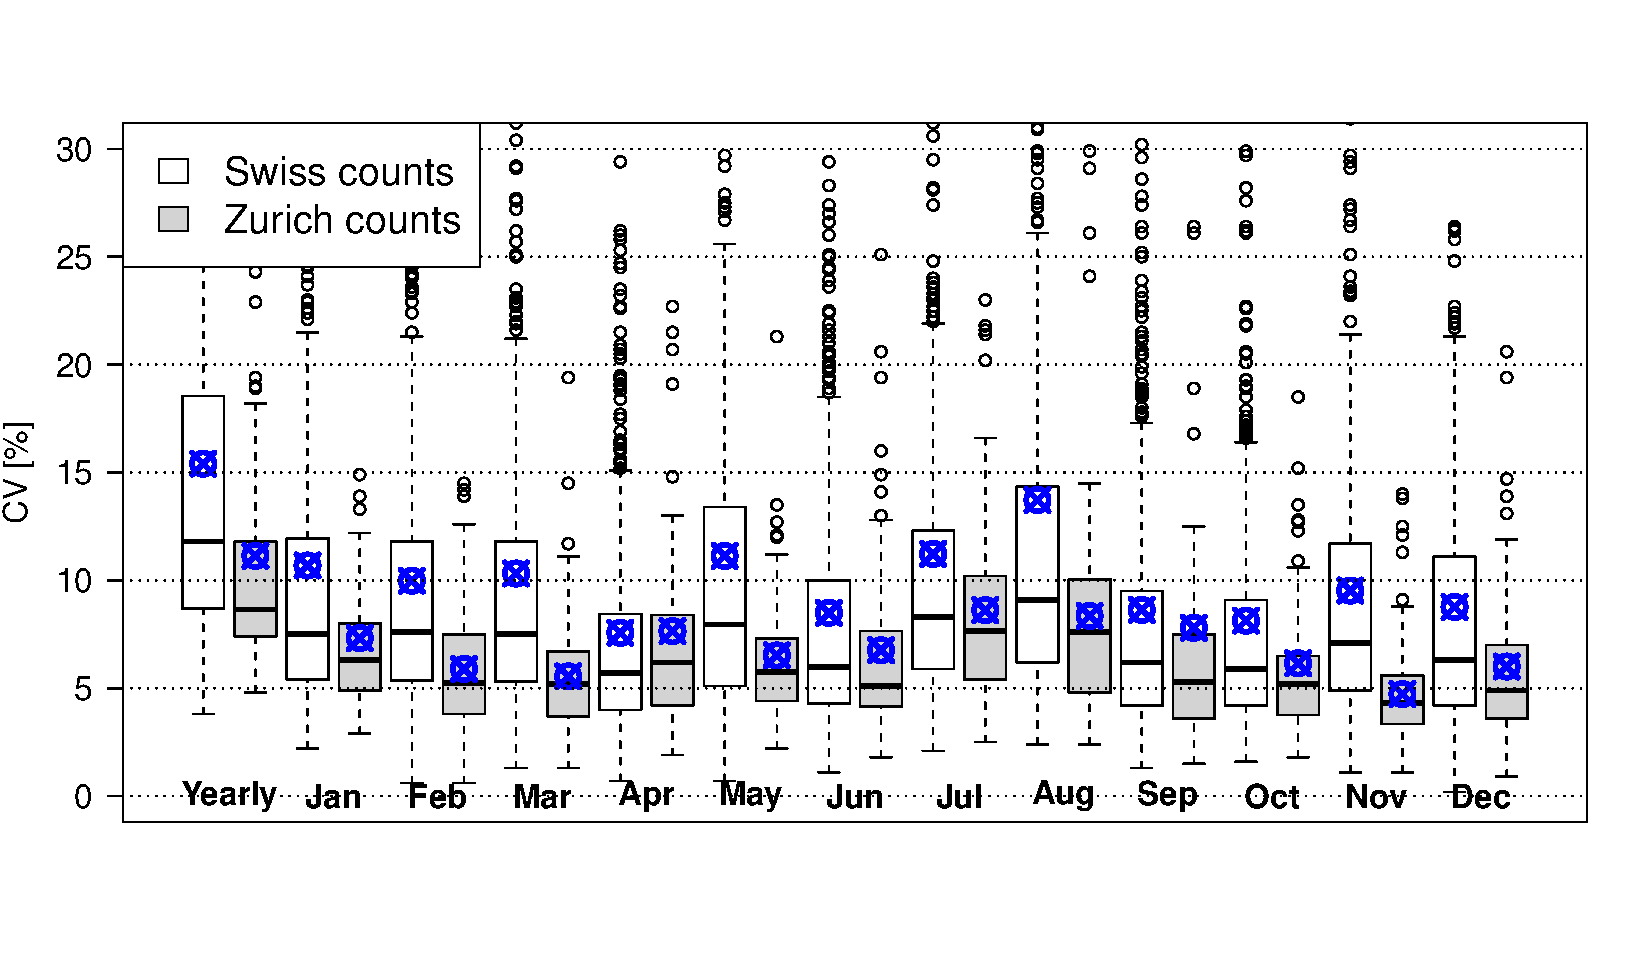
\includegraphics[width=0.8\textwidth]{understanding/figures/var/counts17-18.pdf}}%
	{\label{fig:H1718}}%
  {}%
}%
{}

% ##################################################################################################################
\subsection{Equilibrium}
\label{sec:matsimeq}
Not much is known about the characteristics of the equilibrium found by the MATSim co-evolutionary algorithm. The Nash equilibrium and the Wardrop equilibrium as its instance in transport planning are formulated for unilateral changes. But, in the co-evolutionary algorithm of MATSim, per iteration multiple persons (a specified share of the population) are allowed to modify their plans.

Due to, first, potential individual variations in utility function parameters, second, the implicit unobserved heterogeneity introduced by time and route choice, and third, the explicit error terms applied for destination choices the travelers in MATSim do perceive the travel costs differently. Thus, the equilibrium searched for in MATSim is rather a stochastic than a deterministic user equilibrium. Additionally, it is dynamic. The classification of the MATSim equilibrium as a \emph{Mixed Strategy Nash Equilibrium} (MSNE) is often discussed in personal communications. This type of equilibrium is based on decision-makers which do not chose one specific alternative but a stable probability distribution over the alternatives. 

An argument for the MSNE is as follows. The final state of MATSim with respect to the selected plans in one iteration is never perfectly stable if replanning is turned on and if this replanning is based on random mutation. This is the case for the very common replanning dimension \emph{time choice}. However, this argument is weak as the share of replanners is usually relatively small leading to small intra-run fluctuations. Furthermore, one could specify the result to be based not on the modified selected plan of the current iteration, but on the best plan of each agent. Although the stability of the best plans is not researched extensively, experience tells that for the vast majority of the agents the best plan is stable after having reached the global relaxed state.  

Another argument for the MSNE can be, at first sight, the selection mechanism of MATSim. For some configurations, the plans are selected for replanning and execution according to a logit-type probability distribution. But having a closer look, this argument is also weak. The plans in an agents memory converge all toward the best plan over the course of iterations, as with every replanning stage the worst plan is removed. 

In conclusion, this means that no probability distribution is involved from which the agents draw in the equilibrium state, meaning that the arguments for an MSNE are weak. Clearly, the results over \emph{multiple runs} with different random numbers represent a distribution, but this is not related to the discussion here.

The development of static flow equilibria to dynamic particle equilibria and finally agent-based equilibria is presented in \citet[][]{Nagel_unpub_Latsis_2012, NagelFloetteroed_IATBR_2009}, representing an interesting connection point for a methodological discussion of MATSim system characteristics. Another starting point is provided by \citet[][]{Meister_PhDThesis_2011}, who researched stopping criteria in relation to the MATSim user equilibrium.

%\ah{\citet[][p.509]{NagelBarrett_IJMPC_1997}: Grundidee relaxation procedure schon hier drin! }

% ##################################################################################################################
\subsection{Ergodicity and Emergence}
As mentioned earlier, the driving forces of the transition from non-equilibrium states to an equilibrium and its empirical and behavioral basis are not well understood. If it happened to be the case, that there is no strong driving force, then the maintaining of the assumption of a dominating equilibrium state, would require ergodicity of the system \citep[see also][p.252]{Holden_JTEP_1989}, meaning that the system is actually able to reach all states of the state space. MATSim ergodicity is discussed in \citet[][]{Floetteroed_unpub_MCM_2012}.    

Emergence, the formation of complex patterns generated by interaction of comparatively simple individual units, appear in many systems including transport system. Often, emergent effects are highly significant, such as phantom traffic jams. Consequently, the ability to reproduce them is crucial to modeling these systems. Multi-agent-based simulations are due to their structural similarity to the modeled multi-part systems, expected to be particularly suitable to capture these effects. A glimpse at emergence in MATSim is taken in \citet[][]{HorniMontini_STRC_2013, HorniMontini_TechRep_IVT_2013}. 

% ##################################################################################################################
\subsection{Model Scope}
\label{sec:scope}
Clearly, for most models not the complete range of choice dimensions can be handled endogenously from the beginning, but needs to be fed into the model as input. Successively, during model development, more choice dimensions are included, in \citet[][]{NagelAxhausen_TechRep_IVT_2001} called ``endogenising''. Figure~\ref{fig:scope} loosely derived from \citet[][Figure 2]{NagelAxhausen_TechRep_IVT_2001}) shows the MATSim scope ranging from queue-based traffic flow to demand generation. Time, route, mode and destination choice are endogenously modeled. Activity chains \footnote{Activity chain choice is available in an experimental instance only (Section~\ref{sec:activitychoice}).} and locations for home and work activities are given as model input. Joint activities and rides, sometimes seen as an additional choice dimension, are researched intensively in the context of social networks and households (see Chapter~\ref{ch:jointtrips}). Projects combining MATSim with land use models, here with UrbanSim \citep[][]{NicolaiEtAl_TechRep_VSP_2011, NicolaiEtAl_ERSA_2011, SchirmerEtAl_ERSA_2011, Waddell_unpub_UrbanSimTutorial_2010} are underway (Section~\ref{sec:landuse}).

% ----------
\createfigure%
{Model Scope}%
{Model Scope \kai{Benjamin and I are very strongly for ``macroeconomics'' instead of ``economics'', since economics in general pertains also to route choice, demand generation and land use.}}%
{\label{fig:scope}}%
{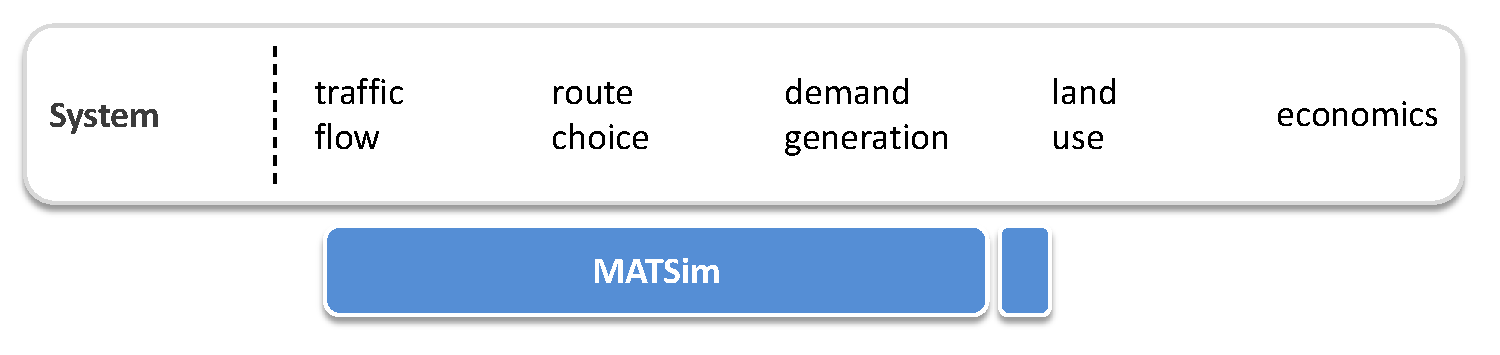
\includegraphics[width=0.99\textwidth, angle=0]{understanding/figures/scope.pdf}}%
{}
%
% ----------

% ##################################################################################################################
%\subsection{Best Response Versus (Weighted) Random Choice}
%\label{sec:bestResponseOrRandom}
%Kai hatte das im Conceptual Meeting angesprochen -> innovative Module müssen keine exakten Lösungen vorschlagen. Diskussion der Unterschiede zu BestResponse (z.B. DC)
%
%Methodische Diskussion:
%route choice -> random walk führt zu nichts
%man könnte best response plus Fehlerterm versuchen
%
%Routing in Hypernetzen? Wie kann man Suchraum begrenzen? -> siehe auch equilibration bei Zielwahl.
%RandomizedRouter (Gauteng) -> siehe Mail von A. Neumann

% ##################################################################################################################
